\subsection{Evaluation of anomaly results}
All three density scoring methods work differently, and the density scoring interval is very different from the probability based to the distance based methods. It is not clear how much deviation in density score is enough to classify an observation as an outlier, but the potential outliers from each method are highlighted in figure \ref{fig:2DdensityPC}.
\begin{figure}[H]
    \centering
    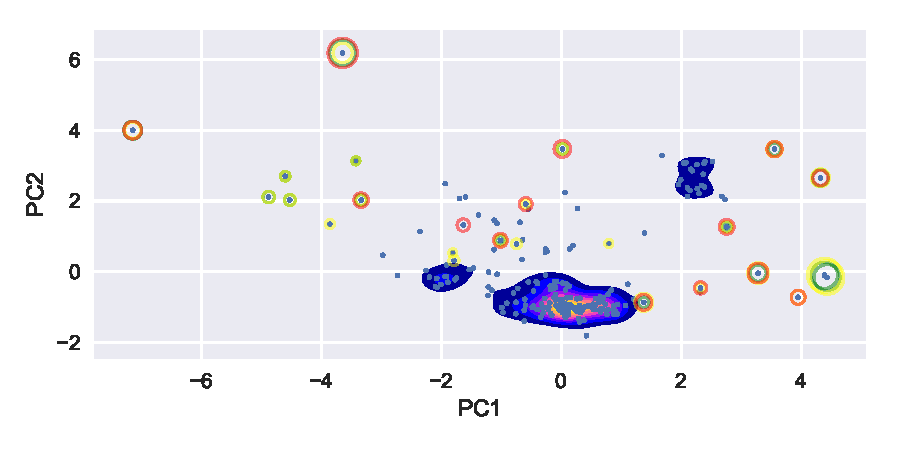
\includegraphics[width=0.7\textwidth]{fig/2DdensityPC.pdf}
    \caption{Potential outliers from each method highlighted with circles, where the radius of the circle correspond to the potential. Color coding: KDE red - KNN green - ARD yellow. A contour plot of the probability function for KDE is shown in the blue heat map. The axes are the first and second PCA components.}
    \label{fig:2DdensityPC}
\end{figure}

The KDE method mainly finds three islands, as seen in blue contour plot in figure \ref{fig:2DdensityPC}, where the density is higher. Especially the lower cluster is highlighted, as expected.

The data set contains observations which are target by all three methods, suggesting these observations are more likely to be outliers for the current data set. A criterion/threshold must be provided in order to directly classify them as anomalies.
%Despite some irregulatities in which observations are chosen as potential outliers, we see several observations which are targeted by all three methods which suggest that the data set indeed contains outliers.

It is also clear that the projection onto the two most principal components does not contain the complete information of the data set, and is only used as a tool for visualization. An observation such as the one just to the right of the main cluster, is seen as more anomalous by all three methods, than the otherwise spread out observations which are not highlighted.